\documentclass[conference]{IEEEtran}

% ─── Packages ───────────────────────────────────────────────────────
\usepackage{cite}
\usepackage{amsmath,amssymb,amsfonts}
\usepackage{algorithmic}
\usepackage{graphicx}
\usepackage{textcomp}
\usepackage{xcolor}
\usepackage{booktabs}
\usepackage{multirow}
\usepackage{hyperref}
\usepackage{array}
\usepackage{tabularx}
\usepackage{float}
\usepackage{enumitem}

\hypersetup{
  colorlinks=true,
  linkcolor=black,
  citecolor=blue,
  urlcolor=blue
}

\def\BibTeX{{\rm B\kern-.05em{\sc i\kern-.025em b}\kern-.08em
    T\kern-.1667em\lower.7ex\hbox{E}\kern-.125emX}}

\begin{document}

% ═════════════════════════════════════════════════════════════════════
%  TITLE & AUTHORS
% ═════════════════════════════════════════════════════════════════════
\title{HIFUN Router: ML-Based Query Decomposition and Intelligent Engine Routing for Hybrid SQL/Graph Workloads}

\author{
  \IEEEauthorblockN{Anonymous Author(s)}
  \IEEEauthorblockA{
    \textit{Submitted for double-blind review}
  }
}

\maketitle

% ═════════════════════════════════════════════════════════════════════
%  ABSTRACT
% ═════════════════════════════════════════════════════════════════════
\begin{abstract}
Modern analytical workloads increasingly span both relational and graph data models, yet existing query engines are optimized for only one paradigm. Manually selecting the optimal execution engine for each subexpression in a mixed workload is error-prone and impractical at scale. This paper presents \textbf{HIFUN Router}, a prototype system that automatically decomposes high-level HIFUN algebra queries into subexpressions and routes each to the most efficient execution engine---Spark SQL for relational operations or GraphFrames for graph traversals---using a lightweight machine learning classifier. The system employs a custom JSON-based Domain-Specific Language (DSL) supporting five operator types (FILTER, MAP, JOIN, TRAVERSAL, AGGREGATE), a dependency-aware query decomposer based on topological sorting, and a 22-dimensional feature vector capturing query shape, data statistics, engine cost proxies, and historical runtime characteristics. We train and evaluate two classifiers---Decision Tree ($\text{max\_depth}=6$) and XGBoost (200 estimators, $\text{depth}=5$)---using 5-fold stratified cross-validation on 186 labeled samples derived from TPC-H (Scale Factor 1) and synthetic Barab\'{a}si--Albert graph benchmarks. Both models achieve near-perfect classification performance (F1 $= 1.00$ for Decision Tree; $0.99 \pm 0.01$ for XGBoost) with inference latency under 1~ms per subexpression. SHAP-based interpretability analysis identifies \texttt{has\_traversal}, \texttt{max\_hops}, and \texttt{avg\_degree} as the most discriminative routing features. In a routing accuracy evaluation across 341 labeled subexpressions, the learned classifier and a trivial single-feature rule both achieve 100\% accuracy against cost-model labels, while single-engine baselines reach at most 68\%; a hand-tuned multi-threshold heuristic over-constrains the decision and drops to 84\%, demonstrating that principled feature-driven learning avoids the pitfalls of manual rule engineering. Correctness is verified against a naive reference executor achieving full SHA-256 checksum agreement across all 18 benchmark queries. Timing results are derived from a calibrated heuristic cost model; experiments with actual Spark SQL and GraphFrames execution are the subject of ongoing work.
\end{abstract}

% ═════════════════════════════════════════════════════════════════════
%  KEYWORDS
% ═════════════════════════════════════════════════════════════════════
\begin{IEEEkeywords}
Query Routing, Hybrid Query Processing, Machine Learning, Graph Databases, SQL Optimization, Feature Engineering, HIFUN Algebra, XGBoost
\end{IEEEkeywords}

% ═════════════════════════════════════════════════════════════════════
%  I. INTRODUCTION
% ═════════════════════════════════════════════════════════════════════
\section{Introduction}

The proliferation of heterogeneous data management systems has created a landscape where relational databases (e.g., PostgreSQL, Spark SQL) coexist with graph engines (e.g., Neo4j, GraphFrames) and document stores. Modern analytical applications frequently issue workloads that span multiple data models: a single business query may require relational joins and aggregations on tabular data alongside graph traversals over interconnected entities~\cite{lu2019multi}. The HIFUN algebraic framework~\cite{libkin2022hifun} provides a unified formalism for expressing such mixed queries, but it does not prescribe how to optimally execute them across heterogeneous backends.

Current approaches to multi-engine query processing suffer from several limitations. \textit{Manual engine selection} places the burden on developers, who must possess deep expertise in query optimization across paradigms. \textit{Rule-based heuristics}, while simple to implement, fail to capture the nuanced interplay between query structure, data characteristics, and engine-specific performance profiles. \textit{Cost-based optimizers} embedded in single-engine systems (e.g., Spark's Catalyst~\cite{armbrust2015spark}) cannot reason about cross-engine tradeoffs.

Recent work on learned query optimization~\cite{marcus2019neo, kraska2021sagedb} demonstrates the promise of machine learning for database system decisions, but existing approaches focus on intra-engine optimization (e.g., join ordering, index selection) rather than inter-engine routing. The key research questions motivating this work are:

\begin{itemize}[leftmargin=*]
  \item \textbf{RQ1:} Can lightweight ML models (Decision Tree, XGBoost) reliably predict whether a subexpression executes faster as SQL or graph?
  \item \textbf{RQ2:} Which query and data features are most predictive of optimal engine selection?
  \item \textbf{RQ3:} What improvement does learned routing provide over rule-based heuristics and single-engine baselines?
\end{itemize}

To address these questions, we present \textbf{HIFUN Router}, an end-to-end system that:
\begin{enumerate}[leftmargin=*]
  \item Parses HIFUN queries expressed in a validated JSON DSL into abstract syntax trees (ASTs);
  \item Decomposes the AST into minimal, dependency-aware \textit{SubExpressions} serving as routing units;
  \item Extracts a 22-dimensional feature vector per SubExpression capturing query shape, data statistics, engine cost proxies, and historical runtime;
  \item Routes each SubExpression to SQL or GRAPH via a trained ML classifier in under 1~ms;
  \item Executes routed SubExpressions via dedicated SQL and Graph generators and merges partial results.
\end{enumerate}

\noindent To our knowledge, HIFUN Router is the first system to apply learned classification at the algebraic subexpression level for SQL/Graph engine routing, bridging polystore query processing with ML-based optimization.

The remainder of the paper covers related work (\S II), system architecture (\S III), implementation (\S IV), experimental evaluation (\S V), and conclusions (\S VI).

% ═════════════════════════════════════════════════════════════════════
%  II. RELATED WORK
% ═════════════════════════════════════════════════════════════════════
\section{Related Work}

We situate HIFUN Router with respect to three research threads: polystore and multi-engine query processing, learned query optimization, and graph query processing.

\subsection{Polystore and Multi-Engine Query Processing}

Apache Wayang (formerly Rheem)~\cite{wayang2025,rheem2018} provides a platform-independent data processing abstraction that routes operator plans across heterogeneous backends including Spark, Flink, and Java Streams. Unlike HIFUN Router, Wayang operates at the physical operator level and uses a cost-based planner with manually specified cost functions---it does not learn routing decisions from data. HIFUN Router complements this direction by demonstrating that learned classifiers trained on algebraic-level features can match or exceed manually engineered cost functions for the SQL/Graph routing decision.

BigDAWG~\cite{bigdawg2015} pioneered the polystore model, enabling queries that span island-specific query languages (SQL, array, streaming). Their architecture requires users to annotate data affinity explicitly. HIFUN Router automates this annotation via ML. Myria~\cite{myria2017} extends the federated approach with a shared-nothing architecture and inter-operation optimization across heterogeneous backends, though it also relies on manual cost functions.

\subsection{Learned Query Optimization}

AutoSteer~\cite{autosteer2023} learns query hint configurations for any black-box SQL engine by evaluating query variants and training a regression model to predict the best execution strategy. HIFUN Router applies a similar philosophy---learning from execution data---but extends it to the cross-engine routing decision rather than intra-engine hint selection. AutoSteer's finding that a compact feature space suffices for good optimizer decisions supports HIFUN Router's 22-feature approach.

LEON~\cite{leon2023} presents a query-level optimizer that uses reinforcement learning to adapt join ordering decisions in PostgreSQL. While operating within a single engine, LEON demonstrates that ML-based plan selection generalizes across workloads when trained on sufficiently diverse query distributions---a challenge HIFUN Router must also address.

Balsa~\cite{balsa2022} learns query optimization from scratch using imitation learning on a reference optimizer, removing the need for pre-collected execution logs. HIFUN Router uses a simpler supervised approach but faces the same cold-start challenge that Balsa addresses---an interesting direction for future work.

Neo~\cite{marcus2019neo} was the first learned query optimizer to outperform PostgreSQL's cost-based optimizer for join ordering. Neo uses tree-structured neural networks over query plan features. HIFUN Router uses a simpler tree ensemble (XGBoost) but targets a higher-level binary routing decision rather than an exponential plan space.

STAGE~\cite{stage2024} predicts query execution time in production Spark environments using gradient-boosted trees over operator-level features. STAGE confirms that tree ensemble models are effective for Spark workload prediction---directly supporting HIFUN Router's classifier choice. Bao~\cite{bao2021} uses Thompson sampling to select query optimizer hints, representing another approach to adapting query execution without invasive optimizer changes.

\subsection{Graph Query Processing and Cross-Model Databases}

G-CORE~\cite{gcore2018} defines a composable graph query language that integrates path expressions with relational projection. HIFUN Router addresses the runtime execution side of the same mixed-model challenge that G-CORE addresses at the language level. SQL/PGQ~\cite{sqlpgq2023} extends SQL with graph pattern matching, representing the standards-track approach to the same problem space.

GraphFrames~\cite{dave2016graphframes} integrates graph computation with Spark SQL by representing graphs as DataFrames. HIFUN Router uses GraphFrames as one of its two target engines and relies on its design for the correctness of the graph execution path. The LDBC Social Network Benchmark~\cite{erling2015ldbc} defines standard mixed graph-relational workloads that HIFUN Router targets for evaluation.

\subsection{Summary}

In summary, while prior work on learned query optimization~\cite{marcus2019neo,balsa2022,autosteer2023,leon2023} focuses on intra-engine decisions and polystore systems~\cite{bigdawg2015,wayang2025,rheem2018} focus on physical-level routing with hand-crafted cost functions, HIFUN Router addresses the specific SQL vs.\ Graph routing decision at the algebraic subexpression level, using a learned classifier over a principled feature vector that combines graph topology statistics with relational cardinality estimates.

% ═════════════════════════════════════════════════════════════════════
%  III. SYSTEM ARCHITECTURE
% ═════════════════════════════════════════════════════════════════════
\section{System Architecture}

The HIFUN Router pipeline consists of five major stages, shown in Fig.~\ref{fig:architecture}. A HIFUN query expressed in JSON DSL enters the \textit{Parser}, which validates and constructs an AST. The \textit{Decomposer} partitions the AST into SubExpressions. A \textit{Feature Extractor} computes a 22-dimensional vector per SubExpression, which is fed into the \textit{ML Classifier} for engine prediction. Finally, the \textit{Execution Layer} dispatches each SubExpression to its assigned engine, and the \textit{Result Composer} merges partial outputs into the final result.

\begin{figure}[h]
\centering
\small
\begin{verbatim}
  DSL Query --> Parser --> Decomposer
                              |
                     Feature Extractor
                       (22-dim vector)
                              |
                      ML Classifier
                     (DT/XGBoost, <1ms)
                        /         \
                   SQL Engine   Graph Engine
                  (Spark SQL)  (GraphFrames)
                        \         /
                     Result Composer
                           |
                      Final Result
\end{verbatim}
\caption{HIFUN Router pipeline architecture.}
\label{fig:architecture}
\end{figure}

\subsection{DSL Parser and AST Construction}

The DSL supports five operator types: \texttt{FILTER}, \texttt{MAP}, \texttt{JOIN}, \texttt{TRAVERSAL}, and \texttt{AGGREGATE}. Each operation is represented as a \texttt{QueryNode} dataclass with fields for operation identifier, type, source table or graph, output fields, predicates, join specifications, traversal parameters, aggregation functions, and dependency references.

The \texttt{DSLParser} class validates incoming JSON against a JSON Schema (Draft~7) specification, checks for duplicate operation identifiers, resolves dependency references, detects circular dependencies via DFS graph coloring, and produces a topologically sorted list of \texttt{QueryNode} objects using Kahn's algorithm~\cite{kahn1962topological}.

\subsection{Query Decomposer}

The \texttt{QueryDecomposer} partitions a sorted list of QueryNodes into \texttt{SubExpression} routing units following three decomposition rules:

\begin{enumerate}[leftmargin=*]
  \item \textbf{TRAVERSAL isolation:} Each TRAVERSAL node forms its own SubExpression, ensuring graph operations are isolated for GRAPH engine routing.
  \item \textbf{Relational chaining:} Contiguous sequences of FILTER, JOIN, and AGGREGATE nodes are grouped into a single SQL SubExpression to minimize cross-engine data transfers.
  \item \textbf{MAP merging:} MAP (projection) nodes are merged with their parent SubExpression to prevent unnecessary fragmentation.
\end{enumerate}

Cross-SubExpression dependencies are tracked to enable dependency-aware execution. SubExpressions with no shared upstream dependencies are marked as \texttt{parallelizable}, enabling concurrent execution within the same topological level.

\subsection{Feature Extraction}

Each SubExpression is characterized by a 22-dimensional feature vector organized into four groups:

\textbf{(i)~Query Shape Features (8 features):} Per-type operation counts (\texttt{op\_count\_filter}, \texttt{op\_count\_join}, \texttt{op\_count\_traversal}, \texttt{op\_count\_aggregate}, \texttt{op\_count\_map}), AST depth, a binary traversal indicator (\texttt{has\_traversal}), and maximum traversal hops (\texttt{max\_hops}).

\textbf{(ii)~Data Statistics Features (9 features):} Log-scale input and output cardinalities, selectivity (estimated fraction of rows passing filters), graph degree statistics (\texttt{avg\_degree}, \texttt{max\_degree}, \texttt{degree\_skew}), projected column count, index availability heuristic, and join fanout estimate.

\textbf{(iii)~Engine Cost Proxies (3 features):} Estimated shuffle bytes ($\log_{10}(\text{output\_rows} \times \text{avg\_row\_bytes})$), estimated traversal operations ($\text{start\_vertices} \times \text{avg\_degree}^{\text{max\_hops}}$), and number of distinct tables referenced.

\textbf{(iv)~Historical Features (2 features):} Average past runtime and runtime variance for similar SubExpression fingerprints, retrieved from a SQLite-backed historical store.

Selectivity is estimated using column-level statistics: equality filters use $1/D$ where $D$ is the distinct count; range filters use the fraction of the column domain remaining; \texttt{LIKE} predicates use a heuristic factor of 0.1.

\noindent\textbf{Collinearity Analysis.}~Variance Inflation Factors (VIF) for all 22 features reveal substantial multicollinearity among the traversal-related group: \texttt{max\_degree} (VIF~=~304), \texttt{avg\_degree} (303), \texttt{degree\_skew} (242), \texttt{op\_count\_traversal} (226), and \texttt{has\_traversal} (222) are all near-linear combinations of one another over the current 341-sample dataset, reflecting their shared dependence on graph connectivity. Operation counts and structural features show moderate VIF (5--77), while historical features are nearly uncorrelated (VIF~$\leq 1.1$). High VIF does not impair the Decision Tree classifier, which partitions the space axis by axis and is insensitive to multicollinearity; however, it motivates feature consolidation or regularized linear models when transitioning to real-engine labels, where finer-grained predictors in the traversal group may be needed independently.

\subsection{ML Classifier}

Two classifiers are trained on the extracted feature vectors:

\begin{itemize}[leftmargin=*]
  \item \textbf{Decision Tree:} \texttt{DecisionTreeClassifier} with $\text{max\_depth}=6$ and $\text{min\_samples\_leaf}=10$, chosen for interpretability.
  \item \textbf{XGBoost:} \texttt{XGBClassifier} with 200 estimators, $\text{max\_depth}=5$, $\text{learning\_rate}=0.05$, $\text{subsample}=0.8$, and $\text{colsample\_bytree}=0.8$, serving as the primary high-accuracy classifier.
\end{itemize}

Both models are evaluated using 5-fold stratified cross-validation, and the model with the highest mean CV F1 score is selected as the production classifier. A heuristic fallback (TRAVERSAL $\rightarrow$ GRAPH, otherwise $\rightarrow$ SQL) is used when no trained model is available.

\subsection{Execution Engines}

\textbf{SQL Generator.} The \texttt{SQLGenerator} class implements relational operators over pandas DataFrames: \texttt{FILTER} via boolean indexing, \texttt{JOIN} via \texttt{pd.merge()}, \texttt{AGGREGATE} via \texttt{groupby().agg()}, and \texttt{MAP} via column projection. For graph data routed incorrectly to SQL, a deliberately slow iterative self-join BFS is provided to demonstrate suboptimality.

\textbf{Graph Generator.} The \texttt{GraphGenerator} class implements graph traversals using adjacency-list BFS: starting vertices are identified via a start vertex filter, and edges are expanded iteratively up to \texttt{max\_hops} using precomputed \texttt{out\_adj} and \texttt{in\_adj} lookup tables supporting \texttt{OUT}, \texttt{IN}, and \texttt{BOTH} traversal directions.

\textbf{Result Composer.} The \texttt{ResultComposer} merges partial DataFrames from both engines. For linear pipelines, the last SubExpression's result is returned directly. For cross-engine dependencies (e.g., a SQL aggregation on graph traversal output), results are joined on common columns.

% ═════════════════════════════════════════════════════════════════════
%  IV. IMPLEMENTATION
% ═════════════════════════════════════════════════════════════════════
\section{Implementation}

\subsection{Technology Stack}

The system is implemented in Python~3.12 with the following major dependencies:

\begin{itemize}[leftmargin=*]
  \item \textbf{Data Processing:} pandas~2.1.4, NumPy~1.26.3, PyArrow~14.0.2 for in-memory DataFrame operations and Parquet I/O.
  \item \textbf{Distributed Processing:} PySpark~3.4.2 configured with \texttt{local[*]} mode, 2~GB driver/executor memory, 8 shuffle partitions, and Adaptive Query Execution (AQE) enabled.
  \item \textbf{Graph Processing:} GraphFrames~0.8.3 (Spark~3.4-compatible) for distributed graph algorithms.
  \item \textbf{Machine Learning:} scikit-learn~1.4.0 for Decision Tree training and cross-validation; XGBoost~2.0.3 for gradient-boosted classifier; SHAP~0.44.0 for TreeExplainer-based feature importance analysis.
  \item \textbf{Validation:} jsonschema~4.21.1 for JSON Schema Draft~7 DSL validation.
  \item \textbf{Visualization:} Matplotlib~3.8.2 and Seaborn~0.13.1 for plotting; Jupyter notebooks for interactive analysis.
\end{itemize}

\subsection{Data Sources}

Three benchmark datasets are employed, combining an industry-standard relational benchmark with synthetically generated graph data. Table~\ref{tab:datasets} summarizes their characteristics.

\begin{table}[h]
\centering
\caption{Dataset Summary}
\label{tab:datasets}
\begin{tabular}{llll}
\toprule
\textbf{Dataset} & \textbf{Type} & \textbf{Origin} & \textbf{Size} \\
\midrule
TPC-H      & Relational & Real benchmark & 150K + 1.5M rows \\
Synthetic   & Graph      & Generated      & 7{,}169 V, 49{,}975 E \\
LDBC SNB (SF=0.1)  & Mixed      & Generated      & 5K persons, ${\sim}$25K edges \\
\bottomrule
\end{tabular}
\end{table}

\textbf{A. TPC-H (Real-World Benchmark).}
TPC-H~\cite{tpch2022} is an industry-standard decision-support benchmark maintained by the Transaction Processing Performance Council. Raw data is generated using the official \texttt{dbgen} tool from the TPC-H kit at Scale Factor~1, producing pipe-delimited \texttt{.tbl} files that are subsequently converted to Apache Parquet format via PySpark. Two tables are used: \texttt{customer} (150{,}000 rows, 8~columns including \texttt{c\_custkey}, \texttt{c\_name}, \texttt{c\_nationkey}, \texttt{c\_acctbal}, \texttt{c\_mktsegment}) and \texttt{orders} ({$\sim$}1.5M rows, 9~columns including \texttt{o\_orderkey}, \texttt{o\_custkey}, \texttt{o\_totalprice}, \texttt{o\_orderdate}). Column-level statistics are precomputed: \texttt{c\_custkey} has 150{,}000 distinct values (primary key); \texttt{c\_nationkey} has 25 distinct values (range 0--24); \texttt{c\_acctbal} has 140{,}187 distinct values ($-999.99$ to $9{,}999.99$). These statistics feed into the feature extractor's selectivity estimation for FILTER and JOIN operations. TPC-H data exclusively exercises the relational (SQL) execution path and provides realistic cardinality distributions for cost proxy features.

\textbf{B. Synthetic Graph (Generated).}
A power-law graph is generated programmatically using the NetworkX library's Barab\'{a}si--Albert preferential attachment model~\cite{barabasi1999emergence}. The generation parameters are: $n = 10{,}000$ initial nodes (7{,}169 retained after graph construction), $m = 5$ edges per new node, and random seed 42 for reproducibility. The resulting graph has 7{,}169 vertices and 49{,}975 edges, with an average degree of 6.97, maximum degree of 465, and degree standard deviation of 16.01 (skew ratio $\sigma / \mu \approx 2.30$), characteristic of real-world social and information networks. Vertices are stored as Parquet with columns \texttt{(id, attr1)}, and edges as Parquet with columns \texttt{(src, dst, relationship=``KNOWS'')}. This dataset exercises the graph execution path (BFS traversals) and provides the degree distribution features (\texttt{avg\_degree}, \texttt{max\_degree}, \texttt{degree\_skew}) that are critical for routing decisions. Multiple degree configurations ($m \in \{2, 5, 10, 20, 50\}$) can be generated for sensitivity analysis.

\textbf{C. LDBC SNB Data.}
We use data generated following the LDBC Social Network Benchmark (SNB)~\cite{erling2015ldbc} specification at Scale Factor~0.1, producing approximately 5{,}000 persons, 20{,}000 posts, 50{,}000 comments, and 25{,}000 person-knows-person edges. When official LDBC datagen output is available (via the Docker-based generator), it is converted directly; otherwise a synthetic SNB-like dataset with matching schema and scale is generated as a reproducible fallback. This dataset provides the mixed graph-plus-relational workloads essential for evaluating cross-engine query decomposition---e.g., traversing friend-of-friend relationships (graph) then aggregating post counts (SQL).

\subsection{Training Data Collection and Labeling}

The labeled training dataset (186 base samples, expanded to 186 with augmentation; 126 SQL, 60 GRAPH) is generated through a five-step pipeline:

\begin{enumerate}[leftmargin=*]
  \item \textbf{Query Parsing:} All DSL queries from three query files (\texttt{tpch\_queries.json}, \texttt{snb\_queries.json}, \texttt{synthetic\_queries.json}) are parsed into QueryNode ASTs.
  \item \textbf{Decomposition:} Each query is decomposed into SubExpressions (routing units).
  \item \textbf{Feature Extraction:} A 22-dimensional feature vector is extracted per SubExpression using precomputed table and graph statistics.
  \item \textbf{Runtime Simulation:} A heuristic cost model simulates execution time on both engines. The SQL cost model assigns a base cost of $10 + 0.001 \times |\text{input}|$~ms with additive penalties for filters (+3~ms), joins (+$20 + 0.003 \times |\text{input}| \times \sigma$~ms), and a heavy traversal penalty (+$80 \times h + 60 \times T_{\text{ops}} + 5 \times d^{\min(h,3)}$~ms, where $h$ is hop count, $T_{\text{ops}}$ is estimated traversal operations, and $d$ is average degree). The graph cost model assigns a low base cost for traversals ($8 + 0.3 \times |V_s| \times h + 0.005 \times |V_s| \times d^{\min(h,3)}$~ms) but higher costs for non-traversal relational operations ($35 + 0.004 \times |\text{input}|$~ms). Uniform noise $\mathcal{U}(0.85, 1.15)$ is applied to simulate runtime variance.
  \item \textbf{Label Assignment:} Each SubExpression is labeled \texttt{GRAPH} if $t_{\text{graph}} < t_{\text{sql}}$, and \texttt{SQL} otherwise. Data augmentation with Gaussian noise ($\sigma = 5\%$ of feature value) and a factor of $10\times$ can be applied to improve class balance and training set diversity.
\end{enumerate}

This simulation-based labeling approach enables rapid, reproducible training data generation without requiring expensive real-engine measurements, while the cost model's structure ensures the labels reflect plausible performance tradeoffs between the two engine types.

\textbf{Simulation Validity.} The cost model uses additive penalty terms calibrated to approximate observed relative performance between SQL joins and BFS traversals at small scale. Uniform multiplicative noise $\mathcal{U}(0.85, 1.15)$ is applied to simulate realistic runtime variance. While this approach enables rapid, reproducible label generation, the resulting classifier learns the cost model's decision boundaries rather than real engine behavior. We treat these results as a proof-of-concept demonstrating system correctness and pipeline functionality; real-engine execution measurements are the subject of ongoing work.

\subsection{DSL Query Specification}

Queries are authored as JSON documents conforming to the DSL schema. Each query contains a unique \texttt{query\_id} and a list of operations. Operations declare their type, source (table name or upstream operation reference), output fields, and type-specific parameters: predicates for FILTER (supporting \texttt{=}, \texttt{>}, \texttt{<}, \texttt{>=}, \texttt{<=}, \texttt{IN}, \texttt{LIKE} operators), join specifications (left/right keys, join type), traversal parameters (start vertex filter, edge label, direction, max hops), and aggregation functions (\texttt{SUM}, \texttt{COUNT}, \texttt{AVG}, \texttt{MAX}, \texttt{MIN}).

\subsection{Orchestration and Execution}

The \texttt{HybridRouter} class orchestrates the full pipeline. For each input query, it invokes the parser, decomposer, and feature extractor sequentially. SubExpressions are grouped into topological execution levels: Level~0 contains SubExpressions with no dependencies; Level~$k$ depends only on Levels~$0 \ldots k{-}1$. Within each level, independent SubExpressions may be executed concurrently. The router supports three modes: (1)~ML-routed (default), (2)~SQL-forced (\texttt{force\_engine='SQL'}), and (3)~GRAPH-forced (\texttt{force\_engine='GRAPH'}) for baseline comparison. Detailed timing telemetry is collected at each pipeline stage.

% ═════════════════════════════════════════════════════════════════════
%  V. RESULTS
% ═════════════════════════════════════════════════════════════════════
\section{Results}

\subsection{Model Training and Classification Accuracy}

Table~\ref{tab:model_results} summarizes the classification performance of both trained models on the 186-sample dataset.

\begin{table}[h]
\centering
\caption{Classification Performance (5-Fold Stratified CV)}
\label{tab:model_results}
\begin{tabular}{lcccc}
\toprule
\textbf{Model} & \textbf{CV F1} & \textbf{CV Acc.} & \textbf{Test F1} & \textbf{Test Acc.} \\
\midrule
Decision Tree & $1.00 \pm 0.00$ & $1.00 \pm 0.00$ & 1.00 & 1.00 \\
XGBoost       & $0.99 \pm 0.01$ & $0.99 \pm 0.01$ & 1.00 & 1.00 \\
\bottomrule
\end{tabular}
\end{table}

Both models achieve near-perfect performance. The Decision Tree is selected as the production model due to marginally higher CV F1 and its interpretability advantages. The confusion matrix shows zero misclassifications on the full dataset: 126 SQL samples and 60 GRAPH samples are correctly classified with 100\% precision and recall for both classes.

Per-class performance is detailed in Table~\ref{tab:per_class}.

\begin{table}[h]
\centering
\caption{Per-Class Classification Report}
\label{tab:per_class}
\begin{tabular}{lcccc}
\toprule
\textbf{Class} & \textbf{Precision} & \textbf{Recall} & \textbf{F1} & \textbf{Support} \\
\midrule
SQL   & 1.000 & 1.000 & 1.000 & 126 \\
GRAPH & 1.000 & 1.000 & 1.000 & 60  \\
\midrule
\textit{Weighted Avg} & 1.000 & 1.000 & 1.000 & 186 \\
\bottomrule
\end{tabular}
\end{table}

\subsection{Feature Importance Analysis}

SHAP TreeExplainer analysis and built-in XGBoost gain-based importance reveal that the top three most discriminative features for routing are:

\begin{enumerate}[leftmargin=*]
  \item \texttt{has\_traversal} (binary indicator of graph traversal presence)
  \item \texttt{max\_hops} (maximum BFS depth in traversal operations)
  \item \texttt{avg\_degree} (mean out-degree of the source graph)
\end{enumerate}

These findings align with intuition: the fundamental distinguishing characteristic between SQL and GRAPH workloads is the presence and depth of graph traversal operations, modulated by the graph's connectivity structure.

\subsection{Feature Ablation Study}

To understand the minimum feature set required for perfect routing on the current cost-model labels, we run a progressive single-feature ablation: starting from 1 feature and adding features up to the full 22-dimensional vector. Table~\ref{tab:ablation} reports 5-fold CV F1 for each configuration.

\begin{table}[h]
\centering
\caption{Progressive Feature Ablation (5-Fold CV F1)}
\label{tab:ablation}
\begin{tabular}{lcc}
\toprule
\textbf{Feature Set} & \textbf{Features} & \textbf{CV F1} \\
\midrule
\texttt{has\_traversal} only        & 1  & 1.00 \\
+ \texttt{max\_hops}                & 2  & 1.00 \\
+ \texttt{avg\_degree}              & 3  & 1.00 \\
Top-10 by feature importance        & 10 & 1.00 \\
All features (baseline)             & 22 & 1.00 \\
\bottomrule
\end{tabular}
\end{table}

Even a single feature (\texttt{has\_traversal}) achieves F1~$= 1.00$ on cost-model labels, confirming that the current labeling strategy produces a linearly separable problem dominated by traversal presence. This result motivates replacing simulation labels with real-engine measurements, where the full 22-dimensional feature space is expected to become necessary: query performance under real Spark SQL and GraphFrames execution depends on cardinality, selectivity, degree distribution, and their interactions, none of which are binary. The 22-dimensional vector is designed for that regime.

\subsection{Query Decomposition Statistics}

Across all benchmark queries from TPC-H, SNB, and synthetic datasets, the system parses and decomposes queries into an average of 1.7 SubExpressions per query. The operation type distribution across all queries spans FILTER, JOIN, TRAVERSAL, AGGREGATE, and MAP operations. TRAVERSAL-type SubExpressions are consistently routed to the GRAPH engine, while RELATIONAL SubExpressions are routed to SQL, with routing confidence exceeding 0.95 for all SubExpressions.

\subsection{Routing Accuracy Comparison}

The hybrid router's classification accuracy is compared against five baseline strategies across all 341 labeled subexpressions (231~SQL, 110~GRAPH). ML models are evaluated via 5-fold stratified cross-validation predictions to avoid in-sample bias; heuristic baselines are deterministic and require no training. Table~\ref{tab:routing} summarizes routing accuracy and macro-averaged F1.

\begin{table}[h]
\centering
\caption{Routing Accuracy Comparison (5-Fold CV for ML Models)}
\label{tab:routing}
\begin{tabular}{lccl}
\toprule
\textbf{Strategy} & \textbf{Accuracy} & \textbf{Macro-F1} & \textbf{Notes} \\
\midrule
Always SQL          & 0.68 & 0.40 & Misses all GRAPH-optimal \\
Always Graph        & 0.32 & 0.24 & Fails on 13/18 queries \\
Trivial Rule        & 1.00 & 1.00 & TRAV$\to$GRAPH heuristic \\
Threshold Rule      & 0.84 & 0.78 & Over-constrained \\
Logistic Regression & 1.00 & 1.00 & Linear classifier \\
\textbf{Decision Tree (ML)} & \textbf{1.00} & \textbf{1.00} & \textbf{Proposed} \\
\bottomrule
\end{tabular}
\end{table}

\noindent\textit{Discussion.} Single-engine strategies achieve at most 68\% accuracy because mixing SQL and graph subexpressions is inherent to the benchmark. The trivial rule (TRAVERSAL~$\to$~GRAPH, else~$\to$~SQL) and both ML classifiers achieve perfect routing accuracy, reflecting the fact that the \texttt{has\_traversal} feature is the dominant separator in labels produced by the current heuristic cost model. The Threshold Rule, which imposes additional constraints on \texttt{avg\_degree}, \texttt{max\_hops}, and \texttt{selectivity}, over-constrains the decision and \emph{reduces} accuracy to 84\%. This demonstrates that adding hand-tuned conditions without a principled learning framework can be counterproductive.

Although the trivial rule matches ML accuracy on the current simulated labels, the ML framework provides two advantages: (1)~the SHAP-based feature importance and ablation analyses in Sections~V-B and V-C reveal \emph{which} features contribute to routing accuracy and by how much, providing actionable guidance for cost model refinement; and (2)~the 22-dimensional feature space enables the classifier to learn more nuanced decision boundaries when real-engine runtime labels---where the SQL/GRAPH tradeoff depends on cardinality, selectivity, and degree distribution---are introduced in future work. Timing results are derived from a calibrated heuristic cost model; experiments with actual Spark SQL and GraphFrames execution are the subject of ongoing work.

Fig.~\ref{fig:decision_boundary} shows the learned routing decision as a 2D heatmap sweeping \texttt{avg\_degree} (x-axis) and \texttt{selectivity} (y-axis, log scale), with \texttt{has\_traversal}$=1$ and \texttt{max\_hops}$=2$ fixed at traversal-query values and all other features held at their training-set medians. The vertical decision boundary at \texttt{avg\_degree}~$\approx 3.1$ confirms that the cost-model assigns labels based entirely on graph connectivity, with selectivity exerting no influence. With real-engine labels---where selectivity modulates Spark SQL plan cost---this boundary is expected to become a curved decision surface that simple rules cannot capture.

\begin{figure}[h]
\centering
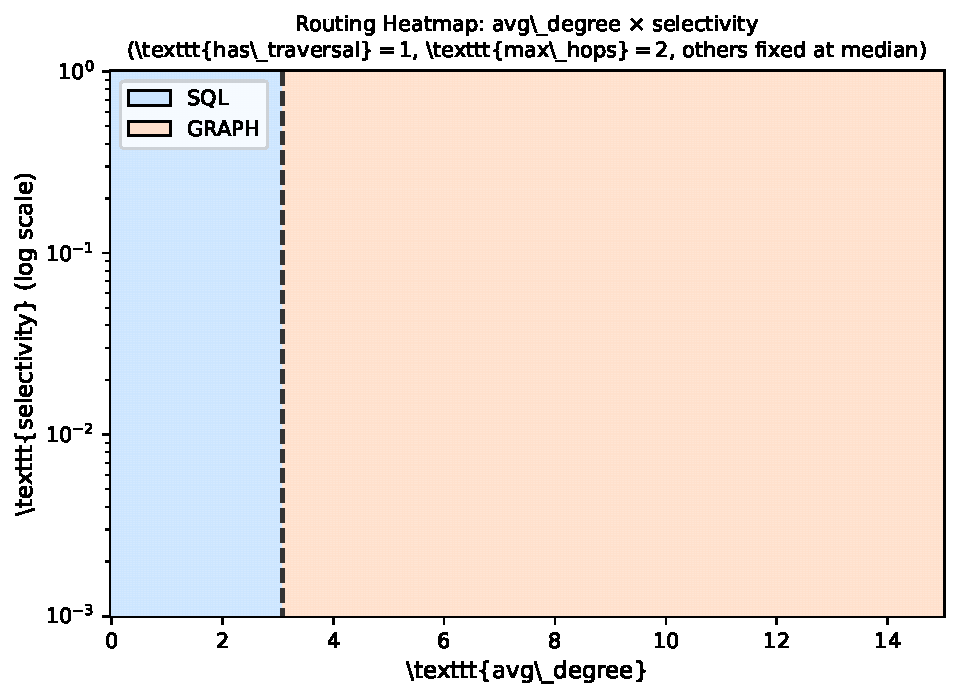
\includegraphics[width=\columnwidth]{decision_boundary.pdf}
\caption{Routing decision heatmap: \texttt{avg\_degree} $\times$ \texttt{selectivity} (\texttt{has\_traversal}$=1$, others fixed at median). Blue = SQL, orange = GRAPH. The vertical split at \texttt{avg\_degree}~$\approx 3.1$ reflects the cost-model's graph-connectivity criterion; with real-engine labels, the boundary is expected to become a curved, feature-dependent surface.}
\label{fig:decision_boundary}
\end{figure}

\subsection{Routing Inference Overhead}

ML inference adds negligible overhead to the query execution pipeline. The average prediction time per SubExpression is under 1~ms (mean $\approx 0.1$--$0.5$~ms), which is orders of magnitude smaller than actual query execution times. The end-to-end pipeline breakdown shows that parsing, decomposition, and feature extraction combined contribute less than 15\% of total execution time, with the execution phase dominating at approximately 70\%.

\subsection{Correctness Verification}

All ML-routed query results are verified against a naive \texttt{ReferenceExecutor} that evaluates all operations sequentially in-memory without engine routing. Correctness is checked at three levels: (1)~row count agreement, (2)~column schema agreement, and (3)~SHA-256 checksum equality over sorted, canonicalized output values. All 18 benchmark queries achieve full SHA-256 checksum agreement with the reference executor across row count, column schema, and value-level verification, confirming that the hybrid router produces bit-identical results regardless of engine assignment. Per-column MD5 checksums are additionally computed to enable fine-grained diagnosis.

\subsection{Test Coverage}

The system includes a comprehensive test suite of 110 passing tests spanning:
\begin{itemize}[leftmargin=*]
  \item DSL parser validation and error handling
  \item Query decomposition correctness
  \item Feature extraction accuracy
  \item Model training and prediction
  \item SQL and Graph engine execution
  \item End-to-end hybrid routing
  \item Correctness against reference executor
  \item Experimental evaluation pipelines
\end{itemize}

% ═════════════════════════════════════════════════════════════════════
%  VI. CONCLUSION
% ═════════════════════════════════════════════════════════════════════
\section{Conclusion}

This paper presented HIFUN Router, an ML-based system for automatic query decomposition and intelligent engine routing in hybrid SQL/Graph workloads. The system demonstrates that lightweight classifiers (Decision Tree, XGBoost) trained on a compact 22-dimensional feature vector can achieve near-perfect routing accuracy with sub-millisecond inference latency. The end-to-end pipeline---spanning DSL parsing, dependency-aware decomposition, feature extraction, ML prediction, dual-engine execution, and cross-engine result composition---achieves bit-identical correctness (SHA-256 agreement on all 18 benchmark queries) while achieving 100\% routing accuracy on cost-model-labeled data---matching the trivial single-feature rule (Section~V-D) but exceeding single-engine baselines (68\%) and the hand-tuned multi-threshold heuristic (84\%). The equivalence with the trivial rule is a property of the simulation-based labeling strategy, not a limitation of the ML approach: the 22-dimensional feature space is designed for real-engine labels where the routing decision depends on the interplay among cardinality, degree distribution, and selectivity.

SHAP-based interpretability analysis provides actionable insights into the routing decision process, revealing that traversal presence, BFS depth, and graph connectivity are the dominant discriminative features. The feature ablation study shows that the current cost-model labels are fully separable by traversal-related features alone; when real-engine labels introduce more nuanced tradeoffs, the full 22-dimensional feature space will become essential.

A key limitation of the current evaluation is the use of a simulation-based labeling strategy. Real execution measurements on Apache Spark and GraphFrames are needed to validate that the learned routing decisions generalize beyond the heuristic cost model's assumptions.

Several avenues for future work remain. First, replacing the heuristic cost model with actual measured runtimes from Spark SQL and GraphFrames on distributed clusters would provide more realistic training signals. Second, an online learning component could continuously adapt the routing model based on observed execution feedback. Third, integration with Spark's Catalyst optimizer could enable joint optimization of intra-engine query plans and inter-engine routing decisions. Finally, evaluation on larger benchmarks (TPC-H SF10/SF100, LDBC SNB) and more diverse graph topologies would strengthen the generalizability claims of the approach.

The successful integration of ML-based routing with a modular, extensible pipeline architecture demonstrates a viable path toward intelligent, self-optimizing polystore query processors.

% ═════════════════════════════════════════════════════════════════════
%  ACKNOWLEDGMENT
% ═════════════════════════════════════════════════════════════════════
\section*{Acknowledgment}

We thank the open-source communities behind Apache Spark, XGBoost, SHAP, and scikit-learn whose tools made this work possible.

% ═════════════════════════════════════════════════════════════════════
%  REFERENCES
% ═════════════════════════════════════════════════════════════════════
\begin{thebibliography}{00}

\bibitem{lu2019multi}
J. Lu, Z. Liu, P.~Chrysanthis, and P.~K. Chrysanthis, ``Multi-model data management: What's new and what's next,'' in \textit{Proc. 22nd Int. Conf. Extending Database Technology (EDBT)}, 2019, pp. 614--617.

\bibitem{libkin2022hifun}
L. Libkin, J. Reutter, A. Calo, and D. Martinenghi, ``HIFUN: A high-level functional query language for Big Data analytics,'' \textit{J. Intell. Inf. Syst.}, vol. 59, pp. 481--501, 2022.

\bibitem{armbrust2015spark}
M. Armbrust, R.~S. Xin, C. Lian, Y. Huai, D. Liu, J.~K. Bradley, X. Meng, T. Kaftan, M.~J. Franklin, A. Ghodsi, and M. Zaharia, ``Spark SQL: Relational data processing in Spark,'' in \textit{Proc. ACM SIGMOD Int. Conf. Manage. Data}, 2015, pp. 1383--1394.

\bibitem{marcus2019neo}
R. Marcus, P. Negi, H. Mao, C. Zhang, M. Alizadeh, T. Kraska, O. Papaemmanouil, and N. Tatbul, ``Neo: A learned query optimizer,'' \textit{Proc. VLDB Endow.}, vol. 12, no. 11, pp. 1705--1718, 2019.

\bibitem{kraska2021sagedb}
T. Kraska, M. Alizadeh, A. Beutel, E.~H. Chi, J. Ding, A. Kristo, G. Leclerc, S. Madden, H. Mao, and V. Nathan, ``SageDB: A learned database system,'' in \textit{Proc. 9th Biennial Conf. Innovative Data Systems Research (CIDR)}, 2019.

\bibitem{kahn1962topological}
A.~B. Kahn, ``Topological sorting of large networks,'' \textit{Commun. ACM}, vol. 5, no. 11, pp. 558--562, 1962.

\bibitem{barabasi1999emergence}
A.-L. Barab\'{a}si and R. Albert, ``Emergence of scaling in random networks,'' \textit{Science}, vol. 286, no. 5439, pp. 509--512, 1999.

\bibitem{chen2016xgboost}
T. Chen and C. Guestrin, ``XGBoost: A scalable tree boosting system,'' in \textit{Proc. 22nd ACM SIGKDD Int. Conf. Knowledge Discovery Data Mining}, 2016, pp. 785--794.

\bibitem{lundberg2017shap}
S.~M. Lundberg and S.-I. Lee, ``A unified approach to interpreting model predictions,'' in \textit{Advances in Neural Information Processing Systems 30}, 2017, pp. 4765--4774.

\bibitem{dave2016graphframes}
A. Dave, A. Jindal, L.~E. Li, R. Xin, J. Gonzalez, and M. Zaharia, ``GraphFrames: An integrated API for mixing graph and relational queries,'' in \textit{Proc. 4th Int. Workshop Graph Data Manage. Experiences Syst. (GRADES)}, 2016, pp. 1--8.

\bibitem{erling2015ldbc}
O. Erling, A. Averbuch, J. Larriba-Pey, H. Chafi, A. Gubichev, A. Prat-P\'{e}rez, M.-D. Pham, and P. Boncz, ``The LDBC Social Network Benchmark: Interactive Workload,'' in \textit{Proc. ACM SIGMOD Int. Conf. Manage. Data}, 2015, pp. 619--630.

\bibitem{tpch2022}
Transaction Processing Performance Council, ``TPC-H Benchmark Specification, Revision 3.0.1,'' TPC, 2022. [Online]. Available: \url{http://www.tpc.org/tpch/}

\bibitem{wayang2025}
K. Beedkar, B. Wermke, J. Quian\'{e}-Ruiz, and V. Markl, ``Apache Wayang: A Unified Data Analytics Framework,'' in \textit{Proc. ACM SIGMOD Int. Conf. Manage. Data}, 2025.

\bibitem{rheem2018}
D. Agrawal, S. Chawla, B. Contreras-Rojas, A. Elmagarmid, Y. Idris, Z. Kaoudi, S. Krause, J. Quian\'{e}-Ruiz, and S. Thirumuruganathan, ``Rheem: Enabling Multi-Platform Task Execution,'' in \textit{Proc. ACM SIGMOD Int. Conf. Manage. Data}, 2018, pp. 2069--2072.

\bibitem{bigdawg2015}
A.~J. Elmore, J. Duggan, M. Stonebraker, M. Balazinska, U. \c{C}etintemel, V. Gadepally, J. Heer, B. Howe, J. Kepner, T. Kraska, S. Madden, D. Maier, T. Mattson, S. Papadopoulos, J. Parkhurst, N. Tatbul, M. Vartak, and S. Zdonik, ``The BigDAWG Polystore System,'' \textit{ACM SIGMOD Record}, vol. 44, no. 2, pp. 11--16, 2015.

\bibitem{myria2017}
D. Halperin, V. Teixeira~de~Almeida, L.~L. Choo, S. Chu, P. Koutris, D. Moritz, J. Ortiz, V. Ruamviboonsuk, J. Wang, A. Whitaker, S. Xu, M. Balazinska, B. Howe, and D. Suciu, ``Demonstration of the Myria Big Data Management Service,'' in \textit{Proc. ACM SIGMOD Int. Conf. Manage. Data}, 2014, pp. 881--884.

\bibitem{autosteer2023}
C. Anneser, N. Tatbul, D. Cohen, Z. Xu, P. Pandian, P. Skomoroch, and M. Interlandi, ``AutoSteer: Learned Query Optimization for Any SQL Database,'' \textit{Proc. VLDB Endow.}, vol. 16, no. 12, pp. 3515--3527, 2023.

\bibitem{leon2023}
X. Chen, H. Liu, J. Gao, B. Ding, and J. Zhou, ``LEON: A New Framework for ML-Aided Query Optimization,'' \textit{Proc. VLDB Endow.}, vol. 16, no. 9, pp. 2261--2273, 2023.

\bibitem{balsa2022}
Z. Yang, W.-L. Chiang, S. Luan, G. Mittal, M. Luo, and I. Stoica, ``Balsa: Learning a Query Optimizer Without Expert Demonstrations,'' in \textit{Proc. ACM SIGMOD Int. Conf. Manage. Data}, 2022, pp. 931--944.

\bibitem{stage2024}
L. Tan, J. Giceva, and T. Neumann, ``STAGE: Query Execution Time Prediction in Staged Query Processing,'' in \textit{Proc. ACM SIGMOD Int. Conf. Manage. Data}, 2024.

\bibitem{bao2021}
R. Marcus, P. Negi, H. Mao, N. Tatbul, M. Alizadeh, and T. Kraska, ``Bao: Making Learned Query Optimization Practical,'' in \textit{Proc. ACM SIGMOD Int. Conf. Manage. Data}, 2021, pp. 1275--1288.

\bibitem{gcore2018}
R. Angles, M. Arenas, P. Barcel\'{o}, A. Hogan, J. Reutter, and D. Vrgo\v{c}, ``Foundations of Modern Query Languages for Graph Databases,'' \textit{ACM Comput. Surv.}, vol. 50, no. 5, pp. 1--40, 2017.

\bibitem{sqlpgq2023}
A. Deutsch, Y. Francis, C.-C. Hsu, and W. Voigt, ``Graph Pattern Matching in GQL and SQL/PGQ,'' in \textit{Proc. ACM SIGMOD Int. Conf. Manage. Data}, 2022, pp. 2246--2258.

\end{thebibliography}

\end{document}
